
\subsection{Large-radius jet mass definitions}

Large-radius jet, or arge-$R$ jets are jets constructed with a radius parameter of the reclustering algorithm much bigger than the standard 0.4; within ATLAS the size of large-$R$ jets is 1.0 for anti-k$_t$ and 1.2 for C/A (the area of C/A is $\sim$20\% smaller than anti-k$_t$).

It is worth noting that, for a standard anti-k$_t$ 0.4 jet the active area \cite{antiktalgo} is $A_{anti-k_t}=\pi R^2 \simeq 0.5$, while it is $\simeq 3.14$ for 1.0 jet, i.e. around six times bigger.

Already from this ``geometrical'' point of view, the necessity of further techniques can be understood: the effect of soft radiation contamination from Pile-Up (PU) and Underlying Event (UE) will be in this case six times bigger and spoil the efficiency of the jet mass measurements.

\subsubsection{Substructure: Grooming Techniques}

This section is based on the 7 TeV article on jet Substructure \cite{substructure1}.
In order to use large-$R$ jets, it is necessary to gain additional information on the interior of these objects, i.e. using techniques that exploit its substructure allowing a jet-by-jet discrimination of the energy deposit most likely coming from the hard-scattering to other soft radiation.

A common feature in substructure is the use of \textit{sub-jet}, i.e. jets obtained from a parent jet (e.g. the large-$R$ jet), using its constituent but running the jet reclustering algorithm with a smaller radius parameter; in one large-$R$ jet, typically there are two or more sub-jets depending on the originating process and its $\pt$.

Techniques have been developed, both using sub-jets or directly constituents of a jet, which are referred to as \textit{grooming} algorithms.

Grooming algorithms are designed to retain the characteristic substructure within such a large-$R$
jet while reducing the impact of the fluctuations of the parton shower and the UE, thereby
improving the mass resolution and mitigating the influence of pile-up.

The grooming algorithms presented here are the most important ones in ATLAS: the \textit{Trimming}; other used as well, the \textit{Split-Filtering} and the \textit{Pruning} can be found in the Appendix.

\subsubsection{Trimming}

The trimming algorithm is the most important in ATLAS and the one mainly used in the work presented in this thesis. It takes advantage of the fact that contamination from soft radiation has a much lower $\pt$ with respect to the hard-scattering component. Therefore uses a transverse momentum balance to distinguish among those. The algorithm works on a two-dimensional parameter space: $R_{sub}$ and $f_{cut}$.
The steps are as follows:
\begin{itemize}
 \item k$_t$ algorithm (but of course other choices are also possible) is used to create sub-jets with a smaller radius $R_{sub}$, aiming at separating the soft radiation from the hard one in different sub-jets. Typical choices are 0.2 and 0.3 (0.2 is used as standard);
 \item for each sub-jet, the ratio $f_{cut}$ of its $\pt$ with the parent jet $p_T^{jet}$ is calculated: if then this ratio is below a certain value, the sub-jet is removed. Standard choice is $f_{cut}=\frac{p_{T}}{p_{T}^{jet}}$=0.05;
 \item the sub-jets which survived this procedure are the only one which compose the trimmed jet.
\end{itemize}

The trimming procedure is also explained in Figure \ref{fig:trimming}, an example of performance in simulation with standard parameters is shown in Appendix (Figure \ref{fig:trimmingperformance}).

\begin{figure}[!ht]
  \centering
      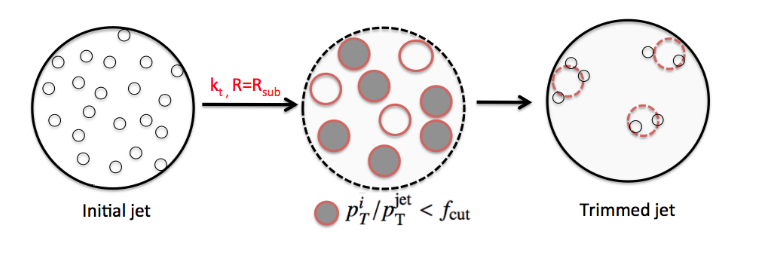
\includegraphics[width=0.9\textwidth]{jet_part/grooming/Figura_4.png}
  \caption{Schematic of the trimming algorithm.}
  \label{fig:trimming}
\end{figure}


\subsubsection{Calorimeter Mass}

% Once the collection of constituents from the large-$R$ jet is groomed, i.e. the most likely sources of soft radiation from PU and UE are eliminated, one can start working with those and start worrying about how to get physical-related properties from it, e.g. the mass.
Once the collection of constituents from the large-$R$ jet is groomed, it is possible to use them for the measure of physical related properties such as the jet mass, since the possible sources of soft radiation from PU and UE have been reduced.


The \textit{calorimeter mass} or $m^{calo}$ is a widely used variable which takes as input the topo-cluster information. Given that each topo-cluster $i$ has a 3D information on the energy deposit, $E_i$, the mass can be simply calculated from 4-vector properties:
$$m^{calo}=\sqrt{\left(\sum_{i\in J}E_i\right)^2-\left(\sum_{i\in J}p_{T,i}\right)^2} $$
where $J$ labels the Large-$R$ jet.

\subsubsection{Track Mass}
\label{sec:tracks}
% This section briefly presents the tracks and how they are related to the properties of the large-$R$ jets.
This section briefly presents the tracks and their relation with the large-$R$ jet's properties.
% There are significant advantages of tracks and why they are interesting and possible candidate for precise mass reconstruction and a big disadvantage.
There are significant advantages and few disadvantages of their usage for precise jet mass reconstruction, which are inherited both from the detector experimental properties and from the underlying physical processes. 

First of all the excellent performance of track reconstruction and angular separation at low $\pt$ is intrinsically better than the calorimeter one (see the Chapter 2. and Table \ref{tab:recap}).
The second main advantage is that tracks can be associated with the primary vertex, thus simply excluding those from PU or other beam-induced soft radiation background (this is not the case for the UE).

The requirement made on tracks to achieve optimal performance are grouped into two categories, the quality of the track, i.e. if it was fully reconstructed from the detector and separated from others with no ambiguities, and the association conditions with the primary vertex:

\begin{itemize}
 \item $p_T^{track} > 400$ MeV;
 \item $|\eta|<$ 2.5;
 \item Maximum 7 hits in the Pixel and STC sub-detectors;
 \item Maximum 1 Pixel hole;
 \item Maximum 2 silicon holes;
 \item Less than 3 shared modules;
 \item Maximum 2 mm of displacement along beam axis ($z_0$) from the primary vertex;
 \item Maximum 2.5 mm of distance in x-y plane from the primary vertex and point of closest approach ($d_0$).
\end{itemize}

Given the set of tracks which pass this selection, the mass $m^{track}$ is calculated summing up the 4-momenta of those tracks which are ghost associated to the groomed jet.

% The main, big disadvantage is that the tracker system is completely blind to the neutral component of the jet, which, as said, amounts to c.a. a third of the total. As seen in Figure \ref{fig:trackandcalo}, the track mass (red distribution) is not only shifted towards lower values than the calorimeter mass (green distribution), but its width also degrades. 

Apart from this benefits which derive from the tracker system, there is also an important disadvantage which comes from the underlying physics: it is completely blind to the electrically neutral component (mostly $\pi^0$) of the jet. As seen in Figure \ref{fig:trackandcalo}, the track mass (red distribution) is not only shifted towards lower values than the calorimeter mass (green distribution), but its width also degrades. 

\begin{figure}[!ht]
  \centering
      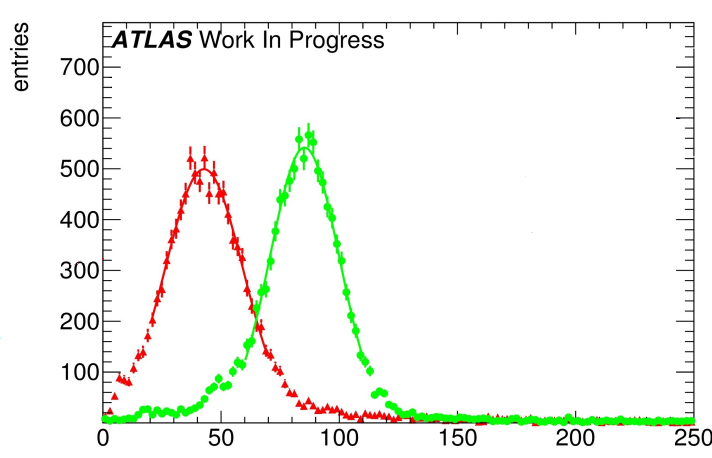
\includegraphics[width=0.7\textwidth]{jet_part/trackandcalo.png}
  \caption[Mass distribution for boosted $W/Z$]{Mass distribution boosted $W/Z$: in green the $m^{calo}$ and in red the $m^{track}$. }
  \label{fig:trackandcalo}
\end{figure}

Tracks could be used either for independent mass reconstruction (and in this section is shown how this is not the case), or, most importantly, as an ulterior information to the calorimeter measurement.

\subsubsection{Performance Figure of Merit (FoM)}
Since we already introduced the calorimeter and track mass, a concrete, quantitative feature has to be defined in order to understand which observable is ``better'', in the sense that we would prefer one or the other according to this criterion. This is often referred to as \textit{Figure of Merit} or simply FoM.

There are few ways to look at the FoM: one can e.g. na\"ively think about the mean of the mass distribution, since closer values of the mean to the e.g. $W$ or $Z$ mass (if we are speaking about $W/Z$ decays), indicate a more correct mass reconstruction. However, this does not take into account the width of this distribution, as a large width spoils the reconstruction in terms of percentage of jets misreconstructed. Moreover, the mean is not as important since it can be rescaled to the desired value in a calibration procedure.

\subsubsection{Gaussian Fit}

The important feature to keep in mind, in fact, is the underlying physics which brings us to calculate the mass of a jet. In figure \ref{fig:search} this is made clear: if the width of the invariant mass distribution of the jet is smaller (highlighted), it allows a bigger background rejection, here shown as the QCD dijet, and a higher signal efficiency, by means of a simple mass requirement.

\begin{figure}[!ht]
  \centering
      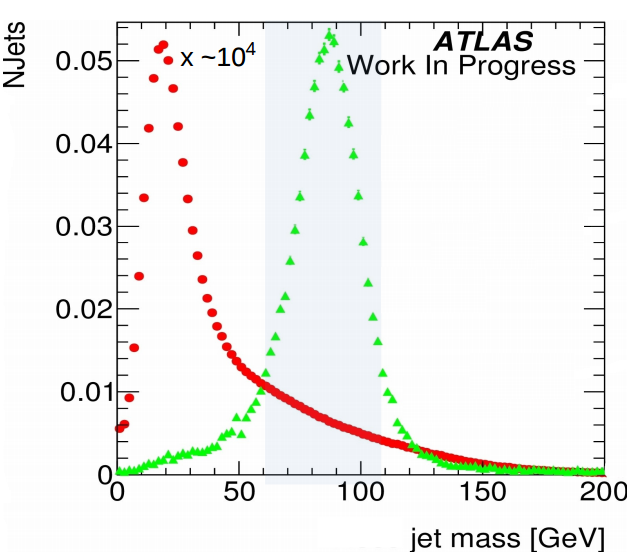
\includegraphics[width=0.55\textwidth]{jet_part/search.png}
  \caption[QCD and $W'$ mass distribution]{Mass distributions: in red the QCD dijet background rescaled, in green the $W/Z$ from the $W'$ sample. Highlighted the width of the $W/Z$ distribution.}
  \label{fig:search}
\end{figure}

The width $\sigma$ of the distribution, which can be obtained from a fit to the Gaussian core, is already a valid FoM, which has an underlying physical feature. Moreover, in order to be independent from the mean of the distribution, the width can be divided by the mean itself.
This was in fact the FoM which was used at the beginning of the work for this thesis, since it provided a simple and fast solution. However, special care must be used both in the procedure of fitting Gaussian cores of responses, since they are asymmetric, and to how the tails are treated.

\begin{figure}[!ht]
  \centering
      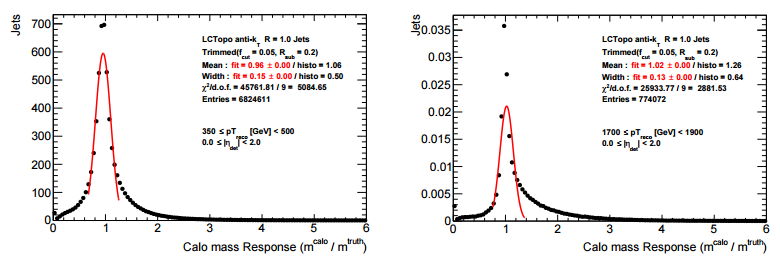
\includegraphics[width=0.9\textwidth]{jet_part/wrongsigma.png}
  \caption[Gaussian fit for QCD multijet]{Mass Response distributions for the QCD multijet for various $\pt$ ranges: on the right the failure of the Gaussian fit shows the limitation of this approach to evaluate the Figure of Merit. On the plot the fit parameters and transverse momentum ranges.}
  \label{fig:wrongsigma32}
\end{figure}

The situation is depicted e.g. in Figure \ref{fig:wrongsigma32}, where a mass response is shown for calorimeter mass for QCD multijet: here the presence of a right-handed tail which enhances going from low to high transverse momenta makes the Gaussian fit clearly not the tool which provides the stability needed. The ideal tool should take care of managing the presence of at least tails outside the Gaussian core and should converge to the intuition of the standard deviation for a perfect Gaussian distribution.
The closest tool to this idea was found to be the \textit{InterQuantile Range}, which was therefore preferred and presented in the next section.

\subsubsection{InterQuantile-Range}
Another way to look at the mass FoM is half of the 68\% of the InterQuantile range (IQnR) (here defined such as it corresponds to a sigma of a ``perfect'' Gaussian distribution: $q84\%-q16\%$ where $q84\%$ is the 84$^{th}$ percentile and $q16\%$ is the 16$^{th}$, not to be confused with the InterQua\textbf{r}tile Range (IQR) which is the $q75\%-q25\%$ and does not correspond to the sigma) divided by the Median ($\iqr$). It provides stability and high sensitivity to left-hand-side and right-hand-side tails.

Another important FoM, used for the work in this thesis, is the response distribution: given the reconstructed mass (calorimeter, track or whichever method) one can compare it to its $truth$ mass ($m^{truth}$), computed from the particle at MC level before the interaction with the detector:

$$R_m=\frac{m^{reco}}{m^{truth}}$$

Standard descriptor of the FoM e.g. in \cite{art35} and here is the IQnR of the $R_m$.
  
  
In Figure \ref{fig:iqrbin} a mass response for a single range of transverse momentum is shown, for the calorimeter mass. On the plot the contours of a standard deviation and of $q16\%$ and $q84\%$ are drawn with dashed and solid lines, respectively, showing the difference induced by the tail. This sort of plot is the key when looking quantitatively to the observable performance and can be found in the Appendix for each of the process studied in every $\pt$ range considered. In this chapter will be shown, however, the quantity which describes this FOM, the IQnR, as a function of $\pt$, in order to get an understanding of the behavior in the entire spectrum and assure the exclusion of local sub-optimalities.

\begin{figure}[!ht]
  \centering
      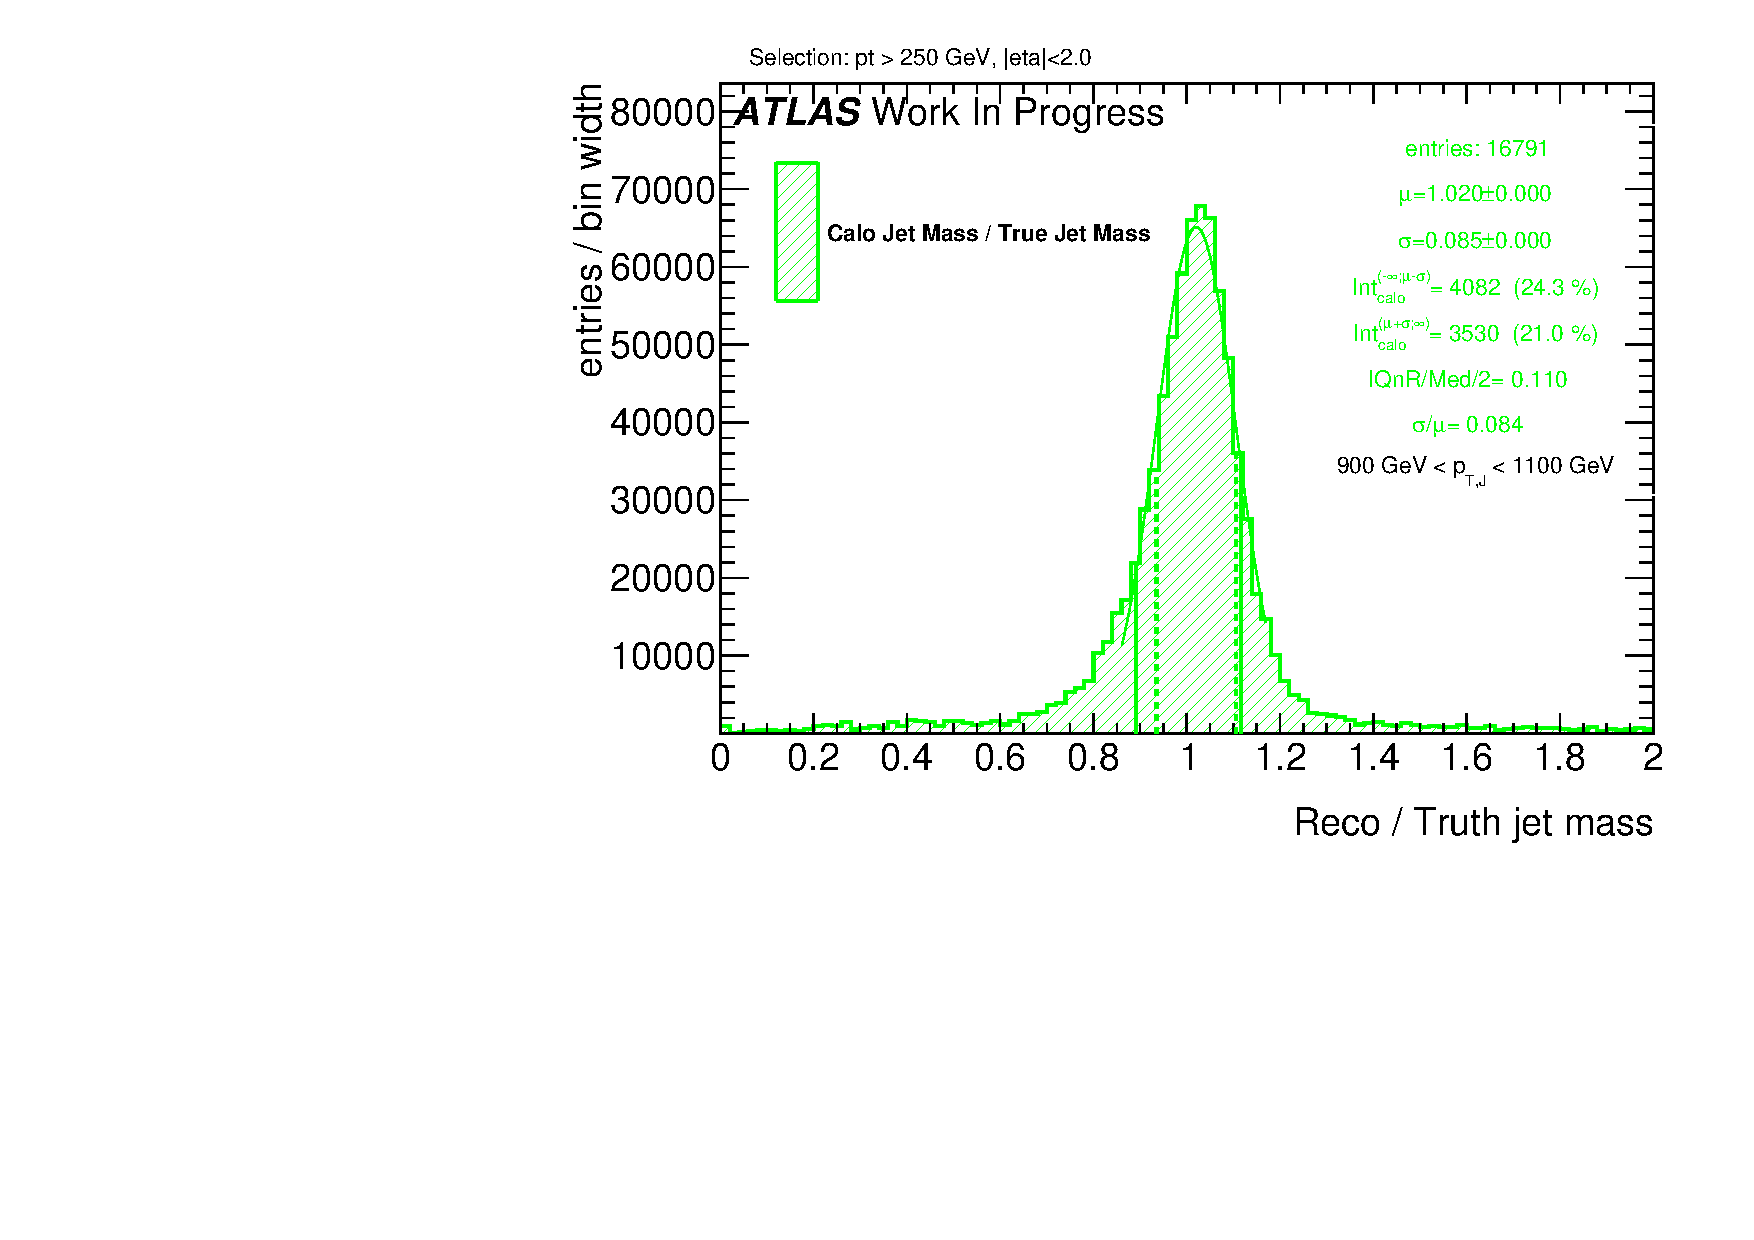
\includegraphics[width=0.7\textwidth]{jet_part/8ResponsePTJ_h_JetRatio_mJ05CALO.pdf}
  \caption[$\mcal$ response single $\pt$ bin]{Calorimeter mass response plot for boosted $W/Z$. One the plot, right, are shown: the number of entries, the mean and the width of the fit to the Gaussian core, the integral from 0 to $\mu-\sigma$ and the one from $\mu+\sigma$ to $+\infty$, the values $\iqr$ and $\sigma/\mu$. On the distribution the dashed vertical lines represent the points $\mu-\sigma$ and $\mu+\sigma$ and the solid lines represent the $q16\%$ and $q84\%$.}
  \label{fig:iqrbin}
\end{figure}